% DSA4212 - Optimisation for Large-Scale Data-Driven Inference
% Small-LLM challenge report. Paste into Overleaf (pdfLaTeX).
% Figures come from analyze.py (analysis/*.png); upload them to Overleaf.
\documentclass[11pt]{article}

\usepackage[margin=1in]{geometry}
\usepackage{graphicx}
\usepackage{booktabs}
\usepackage{amsmath}
\usepackage{siunitx}
\usepackage{hyperref}
\usepackage{caption}

\title{Training a small GPT on TinyStories under a one-hour budget}
\author{Steffany \and Kerem \and Tonio \and [name]\\ \small DSA4212, National University of Singapore}
\date{\today}

\begin{document}
\maketitle

\begin{abstract}
% TODO (write last): 3-4 sentences. Budget, what we varied, the winning config,
% and the single most important trade-off we found.
\end{abstract}

\section{Compute budget declaration}
% TODO: one short paragraph.
\begin{itemize}
  \item \textbf{Budget:} one hour (\SI{3600}{\second}) of in-loop training wall-clock
        \emph{per model}, on identical hardware for every run. Preparation, final
        validation, and checkpointing are outside the timed loop.
  \item \textbf{Hardware:} [GPU / node; from \texttt{run\_config.json} $\to$
        \texttt{runtime.hardware}].
  \item \textbf{From scratch:} random weights (nanoGPT init); no pretrained weights,
        embeddings, or tokenizer fine-tuning.
\end{itemize}

\section{Research question}
We ask: \emph{which model size and training-data fraction gives the best
language-modeling performance under a fixed one-hour budget on identical
hardware?} We hold the tokenizer, optimizer, schedule, context length, and batch
settings fixed and vary only (a) model size and (b) the fraction of the training
split used.

\section{Experimental setup}
\begin{itemize}
  \item \textbf{Data:} \texttt{roneneldan/TinyStories}. Official train split for
        training; official validation split divided 80/20 into validation/test at the
        story level (seed 42). Test used only for the final comparison
        (\S\ref{sec:test}).
  \item \textbf{Tokenizer:} GPT-2 (\texttt{tiktoken}), vocab \num{50257}. Because the
        tokenizer is fixed, per-token loss and perplexity are directly comparable
        across all our runs.
  \item \textbf{Model:} nanoGPT GPT, tied embeddings, causal attention, dropout 0.
\end{itemize}

\begin{table}[h]
  \centering
  \caption{Model sizes compared.}
  \begin{tabular}{lrrrr}
    \toprule
    Size & Layers & Width & Heads & Params (M) \\
    \midrule
    small  & 4 & 256 & 4 & [fill] \\
    medium & 6 & 384 & 6 & [fill] \\
    large  & 8 & 512 & 8 & [fill] \\
    \bottomrule
  \end{tabular}
\end{table}

\noindent\textbf{Data fractions:} 25 / 50 / 75 / \SI{100}{\percent} of the training
split, giving a $3\times4$ grid of 12 runs. \textbf{Optimizer/schedule:} AdamW
(lr \num{3e-4}, wd 0.1, betas 0.9/0.95, clip 1.0), time-based \SI{2}{\percent} warmup
then cosine decay to \SI{10}{\percent} of peak. Context 256, microbatch 16,
accumulation 1.

\section{Methodology and reproducibility}
% TODO: tighten once the runs are done.
\begin{enumerate}
  \item \texttt{python run.py prepare --config configs/default.yaml} builds the token cache.
  \item \texttt{python create\_experiments.py} generates the 12 configs.
  \item Each config trained with \texttt{python run.py train --config \ldots}; outputs in \texttt{results/<name>/}.
  \item Model selected by \emph{validation} loss; only then evaluated on \emph{test}.
  \item \texttt{python analyze.py} aggregates \texttt{results/*/} into \texttt{analysis/}.
\end{enumerate}

\section{Results}
% TODO: paste analysis/summary_table.md converted to LaTeX (or export summary.csv).
\begin{table}[h]
  \centering
  \caption{All runs, sorted by final validation loss. (Paste from \texttt{analysis/summary\_table.md}.)}
  \begin{tabular}{llrrrrr}
    \toprule
    Run & Size & Data\% & Params (M) & Tokens & Val loss & Val ppl \\
    \midrule
    % ...
    \bottomrule
  \end{tabular}
\end{table}

\begin{figure}[h]
  \centering
  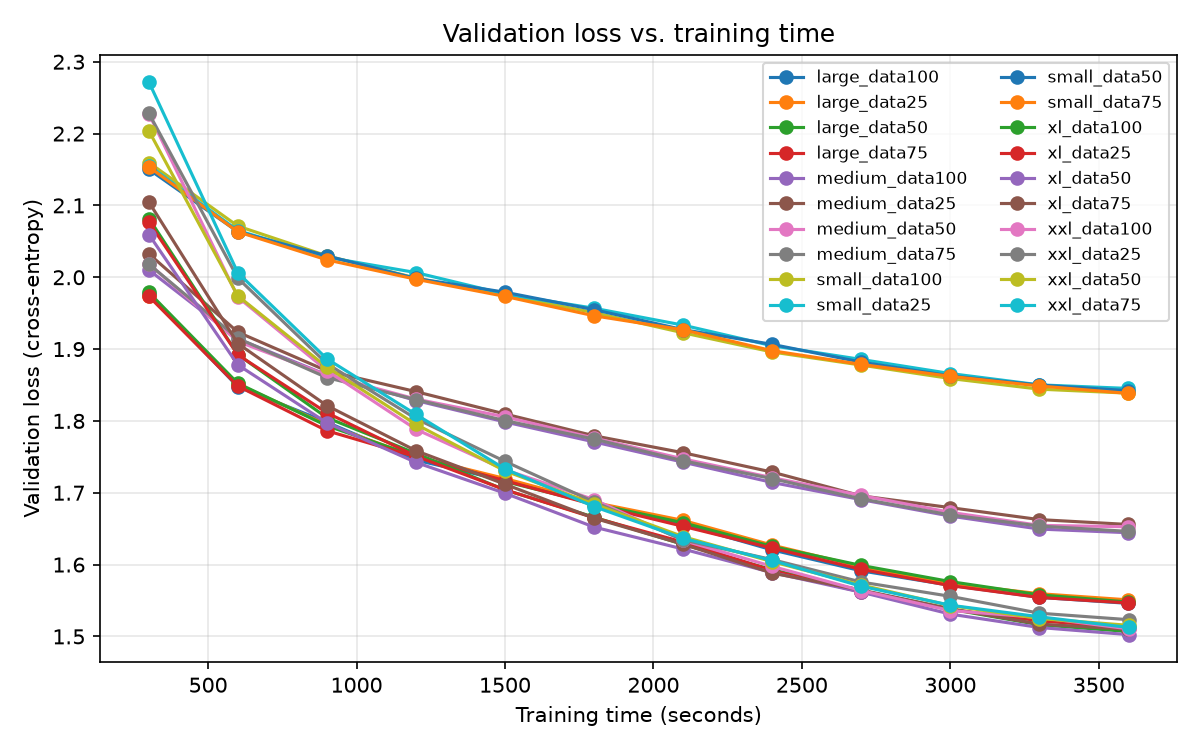
\includegraphics[width=0.7\linewidth]{analysis/val_loss_curves.png}
  \caption{Validation loss over training time. % TODO: which runs converge fastest?
  }
\end{figure}

\begin{figure}[h]
  \centering
  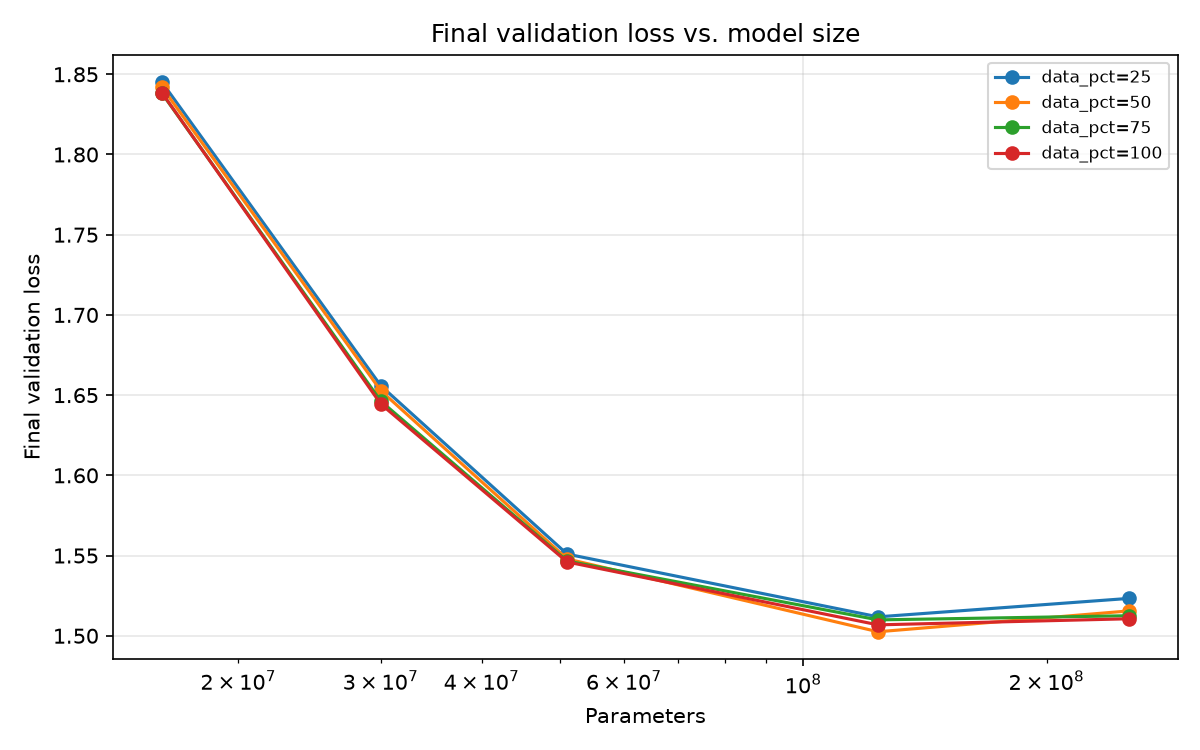
\includegraphics[width=0.49\linewidth]{analysis/val_loss_vs_params.png}
  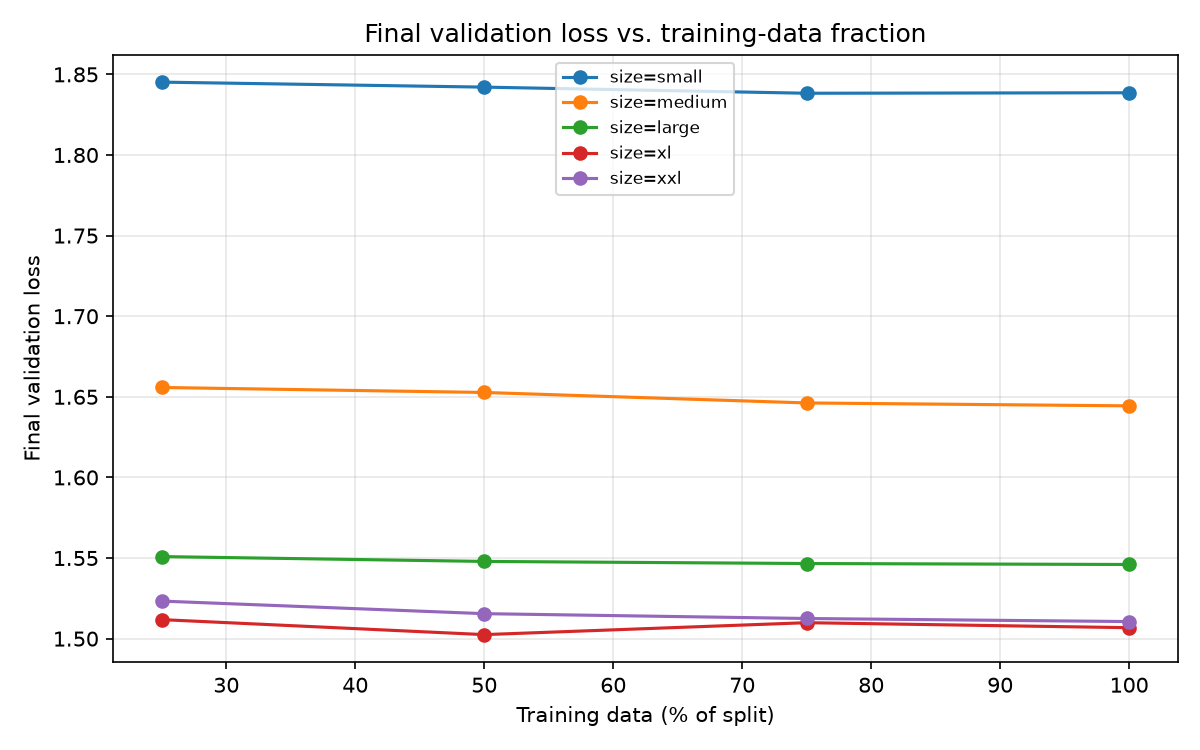
\includegraphics[width=0.49\linewidth]{analysis/val_loss_vs_data.png}
  \caption{Left: final validation loss vs.\ model size (per data fraction). Right:
  vs.\ training-data fraction (per model size). % TODO: interpret.
  }
\end{figure}

\begin{figure}[h]
  \centering
  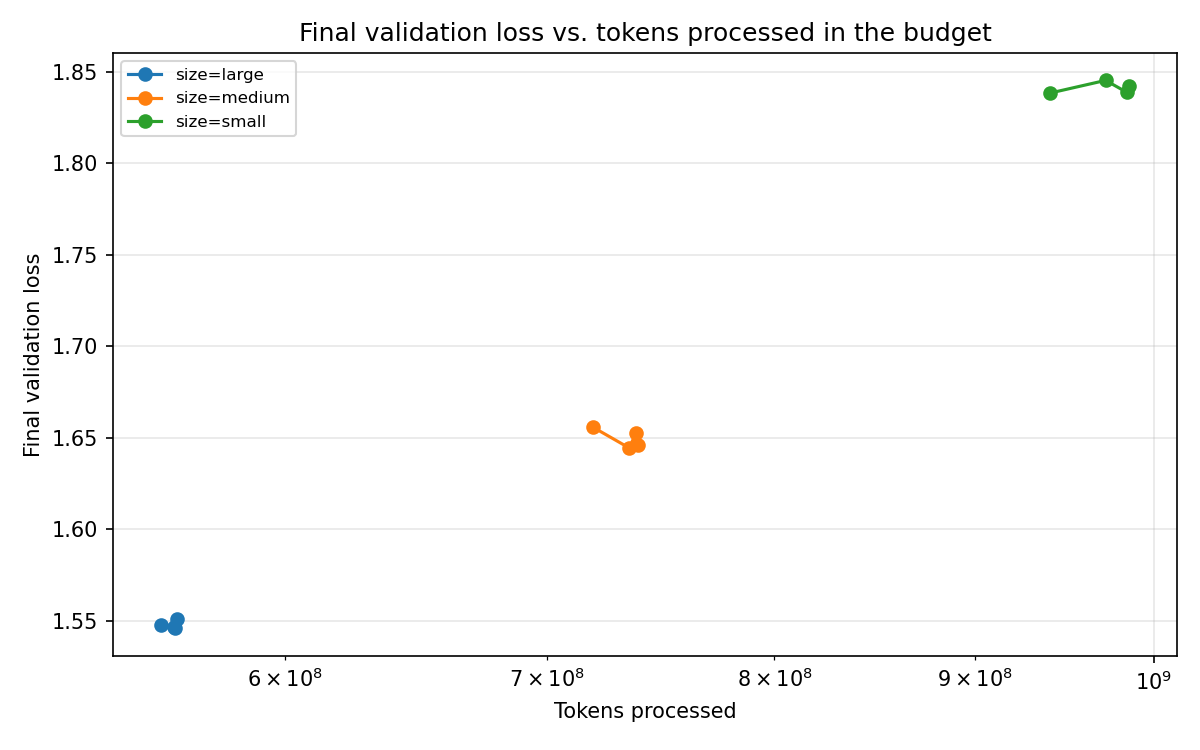
\includegraphics[width=0.49\linewidth]{analysis/val_loss_vs_tokens.png}
  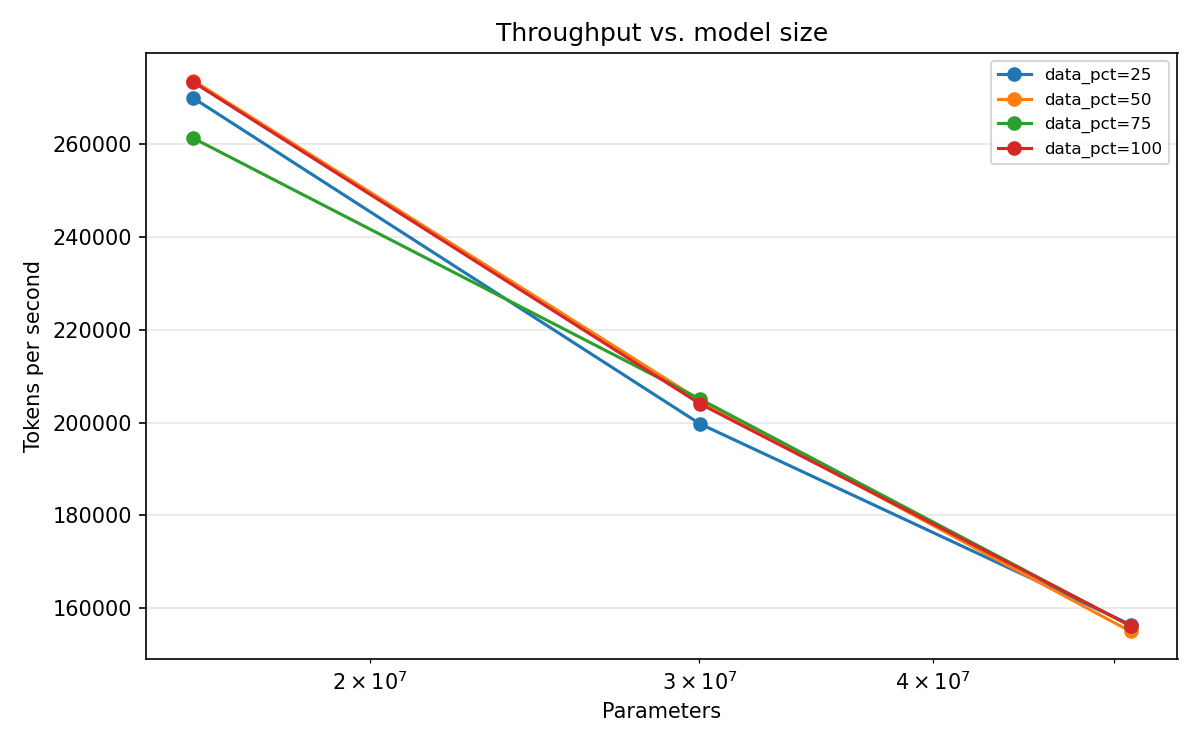
\includegraphics[width=0.49\linewidth]{analysis/throughput_vs_params.png}
  \caption{The core tension: larger models see \emph{fewer} tokens in the same hour.
  % TODO: quantify the trade-off.
  }
\end{figure}

\subsection{Final test result}\label{sec:test}
After selecting the best configuration on validation, its test loss/perplexity is
[fill from \texttt{test\_results.json}]. Only this selected model is evaluated on test.

\subsection{Qualitative evaluation}
% TODO: short rubric scoring of generated stories (grammar, coherence, ends properly).
% Supplements but does not replace the held-out metrics. See appendix for samples.

\section{Discussion}
% TODO: why did the winner win? compute-bound or data-bound? what would change with a
% bigger budget? Limitations: windows sampled with replacement (no guaranteed epoch),
% fixed recipe may not be optimal for every size.

\section{Conclusion}
% TODO: one paragraph answering the research question with the winning config and the
% single most important trade-off.

\appendix
\section{Generated story samples}
% TODO: a few outputs per model from `python run.py generate`.

\end{document}
